% This is "sig-alternate.tex" V1.9 April 2009
% This file should be compiled with V2.4 of "sig-alternate.cls" April 2009
%
% ----------------------------------------------------------------------------------------------------------------
% This .tex file (and associated .cls V2.4) produces:
%       1) The Permission Statement
%       2) The Conference (location) Info information
%       3) The Copyright Line with ACM data
%       4) NO page numbers
%
% as against the acm_proc_article-sp.cls file which
% DOES NOT produce 1) thru' 3) above.
%
% Using 'sig-alternate.cls' you have control, however, from within
% the source .tex file, over both the CopyrightYear
% (defaulted to 200X) and the ACM Copyright Data
% (defaulted to X-XXXXX-XX-X/XX/XX).
% e.g.
% \CopyrightYear{2007} will cause 2007 to appear in the copyright line.
% \crdata{0-12345-67-8/90/12} will cause 0-12345-67-8/90/12 to appear in the copyright line.
%
%
% For tracking purposes - this is V1.9 - April 2009

\documentclass{sig-alternate}

\clubpenalty=300 %10000
\widowpenalty=300 %10000
%\brokenpenalty=1000 %10000

\usepackage{times}

%------------------------------------------------------------------------- 
% take the % away on next line to produce the final camera-ready version 
%\pagestyle{empty}

%------------------------------------------------------------------------- 
\usepackage{arydshln}
\usepackage{boxedminipage}
\usepackage{xspace}
\usepackage{listings}

%Squeeze space in bibliographybg
  \let\oldthebibliography=\thebibliography
  \let\endoldthebibliography=\endthebibliography
  \renewenvironment{thebibliography}[1]{%
    \begin{oldthebibliography}{#1}%
      \setlength{\parskip}{0ex}%
      \setlength{\itemsep}{0ex}%
  }%
  {%
    \end{oldthebibliography}%
  }

\lstset{language=C}


\newcommand{\code}{\tt \small}

\newcommand{\comment}[1]{{}}
\newcommand{\note}[1]{{\bf *** MYTODO: {#1} ***}}


\begin{document}
%
% --- Author Metadata here ---
\conferenceinfo{MSR}{'11 Honolulu, Hawaii, USA}
%\CopyrightYear{2007} % Allows default copyright year (20XX) to be over-ridden - IF NEED BE.
%\crdata{0-12345-67-8/90/01}  % Allows default copyright data (0-89791-88-6/97/05) to be over-ridden - IF NEED BE.
% --- End of Author Metadata ---

\title{When And Why A Bug Is Introduced}
%% \subtitle{Subtitle Text, if any}


%\title{Alternate {\ttlit ACM} SIG Proceedings Paper in LaTeX
%Format\titlenote{(Produces the permission block, and
%copyright information). For use with
%SIG-ALTERNATE.CLS. Supported by ACM.}}
%\subtitle{[Extended Abstract]
%\titlenote{A full version of this paper is available as
%%\textit{Author's Guide to Preparing ACM SIG Proceedings Using
%\LaTeX$2_\epsilon$\ and BibTeX} at
%\texttt{www.acm.org/eaddress.htm}}}
%
% You need the command \numberofauthors to handle the 'placement
% and alignment' of the authors beneath the title.
%
% For aesthetic reasons, we recommend 'three authors at a time'
% i.e. three 'name/affiliation blocks' be placed beneath the title.
%
% NOTE: You are NOT restricted in how many 'rows' of
% "name/affiliations" may appear. We just ask that you restrict
% the number of 'columns' to three.
%
% Because of the available 'opening page real-estate'
% we ask you to refrain from putting more than six authors
% (two rows with three columns) beneath the article title.
% More than six makes the first-page appear very cluttered indeed.
%
% Use the \alignauthor commands to handle the names
% and affiliations for an 'aesthetic maximum' of six authors.
% Add names, affiliations, addresses for
% the seventh etc. author(s) as the argument for the
% \additionalauthors command.
% These 'additional authors' will be output/set for you
% without further effort on your part as the last section in
% the body of your article BEFORE References or any Appendices.

\numberofauthors{1} %  in this sample file, there are a *total*
% of EIGHT authors. SIX appear on the 'first-page' (for formatting
% reasons) and the remaining two appear in the \additionalauthors section.
%
\author{
% You can go ahead and credit any number of authors here,
% e.g. one 'row of three' or two rows (consisting of one row of three
% and a second row of one, two or three).
%
% The command \alignauthor (no curly braces needed) should
% precede each author name, affiliation/snail-mail address and
% e-mail address. Additionally, tag each line of
% affiliation/address with \affaddr, and tag the
% e-mail address with \email.
%
% 1st. author
\alignauthor
Jon Eyolfson, Abdel M. Tawakol\\ 
       \affaddr{University of Waterloo} \\
       \affaddr{200 University Avenue West}\\
       \affaddr{Waterloo, ON N2L3G1, Canada} \\ 
       \affaddr{\em \{jeyolfso, amtawako\}@uwaterloo.ca}
}



\maketitle

%% \category{CR-number}{subcategory}{third-level}

%% \terms
%% term1, term2

%% \keywords
%% runtime monitoring, verification, tracematches, dynamic binary translation

\maketitle

\begin{abstract}
\comment{In this paper we attempt to find a correlation between the commit time
of a code change and the rate of introduction of bugs. In other words,
are developers more prone to bug-inducing changes during certain hours
of the day or not. Before we start our search we were expecting our
results to show that before lunch hour, in anticipation of going for
lunch, and towards the end of the working day in anticipation of going
home. Previous studies have explored whether there is a correlation
between the bug-inducing changes rate and the day of the week, various
mining techniques of bug-inducing changes, but to our knowledge no
work has been to try and find a specific time slots during the day
when developers might be more likely to introduce bugs. We mined data
from Linux and Firefox using their software repositories. We developed
an automated method for extracting information which finds a patch
containing a fix and links it to patches which introduced the bug,
which required the fix. We found the false positive rate to be under
20\% after randomly sampling 100 reports. Our study has found that Thursday is a bad day to code, while
Mondays are surprisingly good. Also between 12AM and 9AM, developers are more prone
to introducing errors, while the least amount of bugs are introduced between
11AM and 3PM. Our data also shows that daily committers are less prone to introducing
bugs, while day-job users are more prone. Finally, the bug lifetimes seem to decay
exponentially, and on average is longer for larger projects.}
\end{abstract}



% There's nothing stopping you putting the seventh, eighth, etc.
% author on the opening page (as the 'third row') but we ask,
% for aesthetic reasons that you place these 'additional authors'
% in the \additional authors block, viz.
\additionalauthors{}
%\date{30 July 1999}

% Just remember to make sure that the TOTAL number of authors
% is the number that will appear on the first page PLUS the
% number that will appear in the \additionalauthors section.


% A category with the (minimum) three required fields
%\category{}{}{}[]
%\category{}{}{}[]

%\category{H.4}{Information Systems Applications}{Miscellaneous}
%A category including the fourth, optional field follows...
%\category{D.2.8}{Software Engineering}{Metrics}[complexity measures, performance measures]

%\terms{Theory}

%\keywords{Empirical Study, Bug detection}


%------------------------------------------------------------------------------



\input intro
\input methods
%\input idea % idea, design, and methods
\input results
\input related
\input conclusions



%\section{Introduction}

The area of bug detection and resolution is currently a very active area of research
in the software related disciplines. The process of detecting and resolving software
bugs is an extremely costly process because of the manpower required to perform
quality assurance on the developed software and having developers perform the fixes.
It is estimated that 20\% - 30\% of the time spent on a software project is spent on
testing and integration \cite{2004-industry}. In addition to the cost of manpower,
the time required to complete these tasks can be costly on the release date of the
software. As such, for the majority of software companies, the process of quality
assurance is costly and time consuming. To put the cost into perspective, a study
conducted by the National Institute of Standard and Technology in 2002 reported that
software bugs cost the economy of the United States approximately \$59.5 billion
annually \cite{2002-economic}. The study also showed that approximately 64\% of
the costs of software bug fixes are incurred by the end users, making this issue
of extreme importance for the consumers as well \cite{2002-economic}.

In our paper we will show the data collected from two large projects, which
are complex and representative of most software projects, namely Linux and Firefox.
Our data includes: percentage of bugs introduced vs total percentage of commits for
every day of the week, percentage of bugs introduced every hour vs percentage of total commits
every hour, percentage of introduction vs percentage of total commits by author classification,
percentage of bugs introduced vs percentage of total commits grouped by author experience,
and bug lifetime.

Our paper does not focus on solving a problem, but instead tries to find correlations between
bug introductions and days of the week, hours of the day, commit introductions by author
experience, commit introductions by author classification, and bug life time. This information
can be used to try and reveal any potential correlations that could help leaders
in the software industry determine ways to minimize any potential effects
of working on a certain day, or during a certain hour. Collecting and analyzing
data with regards to bug introduction will surely be beneficial to reducing bug
introduction rates by examining some of the potential causes.

This paper will be organized in the following fashion: Section
\ref{sec-idea} will give an insight to our idea and how we approached
the problem, Section \ref{sec-impl} discusses our implementation for
automatically finding bug introduction points, Section
\ref{sec-results} presents the results we found, Section
\ref{sec-related} will discuss the related academic work which our
work compliments, Section \ref{sec-future} explores possible future
work, and finally Section \ref{sec-conclusion} concludes our work.


%\input{design}
%- find the commits which fixed a bug
- a bug is an _
- work backwards to find the commits which introduced the bug (ignore merge commits)
 - using the diff information
 - talk about additions/removals/modifications
 - blame
- talk about which type of data we collect
 - author information
 - commit information which

Our goal is to find commits which fix a bug, along with the commits
which introduced that bug. First, we detect a bug-fixing commit $c$ by
searching the commit messages for common keywords such as ``fix'' and
``bug''. Next, we work backwards to locate the commits that introduced
the bug fixed in $c$. Using commit $c$ as a starting point, we compute
a diff for each file between the version after $c$ and the previous
version of that file, and record the line numbers changed in
$c$. Finally, we use the repository metadata to find the commit(s)
$c'$ which were responsible for the previous versions of the files
which were fixed, and we conclude that the commits $c'$ introduced the
bug.

Note that any change in $c$ which removes or modifies an existing line
of code is easy to attribute to a previous commit $c'$, since the
affected line of code existed in $c'$. However, a change in $c$ which
adds a new line of code has no corresponding change in any previous
revision, since this line did not previously exist. In that case, we
attribute responsibility to the commit which introduced the line just
before the new line.

\paragraph{Data collected.}
Executing the above algorithm gives us data about each commit, as well
as the authors of the commits\footnote{Name/email.}.  We record the
following data for each commit: author, time, number of lines changed,
and number of times the commit introduced a bug later corrected. For
each author, we record the name, email(s), experience and
classification.

We compute an author's experience and classification based on the
frequency and duration of that author's commits to a project. Author
experience counts the time between an author's earliest and latest
commits. Author classification describes the author's most-common
frequency between consecutive commits: daily, weekly, monthly, and
single. Note that, for author classification purposes, we ignore
consecutive commits within 30 minutes of each other. As a sub-class of
the daily commiter classification, we also use a heuristic to identify
commiters who worked on the repository as part of their day job,
namely those for which 85\% of commits are between 8 AM and 4 PM
Monday to Friday.

% TODO: manual inspection, bug lifetime

* time zone information

%\section{Results}
\label{sec-results}
In this section, we present the results obtained from carrying out our
methodology, and discuss some of the implications of our results.
Most of our results investigate the effect of an independent variable
(time-of-day and developer experience/frequency classifications) on
the likelihood of a commit to be a bug-introducing commit, or
\emph{bugginess}. We also
describe our findings with respect to the day of the week, which
allows us to compare our results to those
in~\cite{sliwerski-msr-2005}.  Finally, we explain the precision and
recall of our methodology and how we computed these figures.

\paragraph{Project characteristics}
We chose two large open-source software repositories for our
investigations: Linus Torvalds's mainline Linux kernel, from
\url{git.kernel.org} and PostgreSQL, from the project's repository at
\url{git.postgresql.org}. 


Table~\ref{tab:characteristics} summarizes
the characteristics of each of our repositories. 
Row ``bug-introducing'' shows that 23.7-25.5\% of the commits are buggy, which 
is slightly lower than the previously reported nearly 40\% for a commercial switching system~\cite{smallCommits05}. 
%of the samll commits are buggy, this number is on all commits
%in the previous work by Purushothaman and Perry~\cite{smallCommits05}.
Note that the
PostgreSQL repository was carefully converted from CVS using {\code cvs2git} in
September 2010. We discussed some of the quirks of the PostgreSQL repository
in Section~\ref{sec:method}.


\begin{table}
\begin{tabular}{l|r|r}
& {\bf Linux} & {\bf PostgreSQL} \\ \hline
First commit & April 16, 2005 & July 9, 1996 \\
Cloned & November 21, 2010 & January 24, 2011 \\
Lines of code at tip & over 5 million & over 750,000 \\
%Source & \url{git.kernel.org} & \url{git.postgresql.org} \\
Number of authors & 8,594 & 34 \\
Number of commits & 222,332 & 31,098 \\
\# bug-introducing & 56,681 (25.5\%) & 7,366 (23.7\%) \\
\# bug-fixing & 57,028 & 4,399
\end{tabular}
\caption{\label{tab:characteristics}Characteristics of the Linux kernel and PostgreSQL repositories.}
\end{table}

%% The Linux repository
%% was cloned on November 21, 2010, from Linus Torvalds's mainline
%% kernel, hosted at \url{git.kernel.org}; this repository contains
%% history back to April 16, 2005.  This repository contains 222,332
%% commits contributed by 8,594 authors. Of these commits, we identified
%% 56,681 bug-introducing commits and 57,028 bug-fixing commits.
%% The tip of the repository contains
%% over 5 million lines of code. 

%% The PostgreSQL repository was cloned on January 24, 2011, from the
%% project's repository at \url{git.postgresql.org}; it contains history
%% to July 9, 1996, translated from CVS using \code{cvs2git}.  This
%% repository contains 31,098 commits contributed by 34 authors. We
%% identified 7,366 bug-introducing commits and 4,399 bug-fixing commits. The tip
%% of the repository contains over 750,000 lines of code.

\subsection{Time-of-day Results} 
We first present our results correlating the time-of-day of a commit
with its bugginess.  Figures~\ref{fig-linux-bugginess-hour}
and~\ref{fig-postgresql-bugginess-hour} present results from the Linux kernel and
Postgres, respectively. These graphs compare the time-of-day of each
commit, in the committer's local time on a 24-hour clock, to the
percentage of commits which were found to be bug-introducing. The
solid horizontal line indicates the mean number of buggy commits in
each project; bars shorter than the line indicate that commits at that
hour were less likely to be buggy, while bars taller than the line
indicate hours with more-buggy commits. The graphs also contain the
raw number of commits at each hour, as indicated by the red dots.

Both figures show a noticeable increase in the amount of commits which
introduce a bug between 00:00 (midnight) and 04:00 (4AM). After 04:00,
commits tend to be less buggy than average, gradually increasing until
noon.  In the Linux kernel, commits between noon and midnight fluctuate around
the average bugginess level, while the Postgres commits are generally
above the average bugginess level between 16:00 (4PM) and 20:00 (8PM),
and then below the average bugginess level between 20:00 (8PM) and
00:00 (midnight). Note that even the smallest total number of commits,
for any hour, is 139 for Postgres (and an order of magnitude higher
for the Linux kernel), so that all of the depicted bug introduction rates are
meaningful.

Our results suggest that tired developers (midnight-4AM) are more
likely to miss corner cases in a pre-commit review (for Postgres) or
while finalizing the patch (for the Linux kernel). Furthermore, we can observe
that commits before noon are least likely to be bug-introducing;
perhaps committers are most careful in those hours.

\begin{figure}
\begin{center}
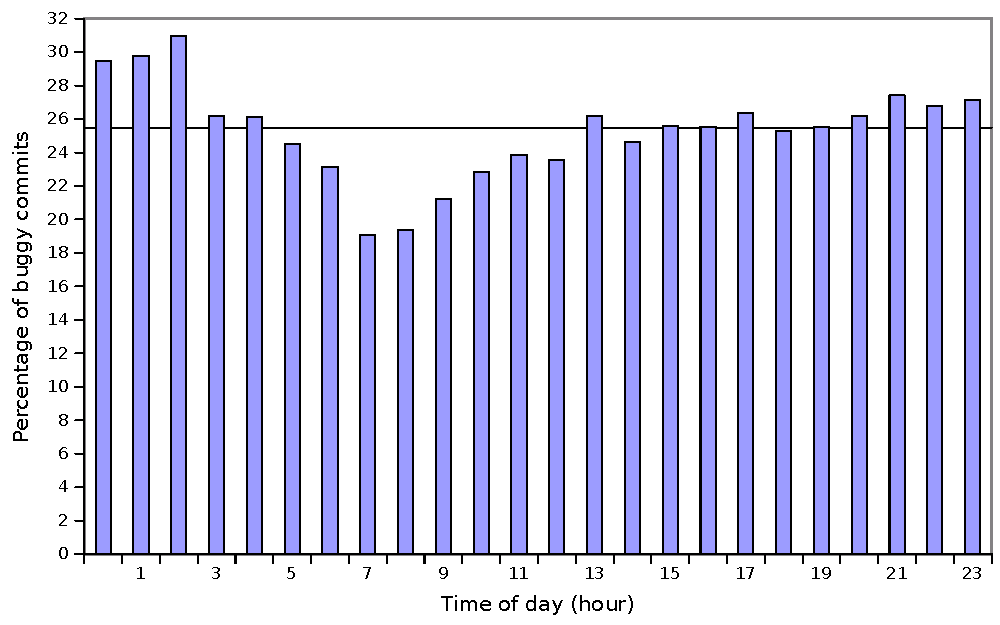
\includegraphics[width=\columnwidth]{linux-bugginess-hour.pdf}
\end{center}
\caption{The Linux kernel percentage of buggy commits (bars) and total number of commits (circles) versus time of day}
\label{fig-linux-bugginess-hour}
\end{figure}

\begin{figure}
\begin{center}
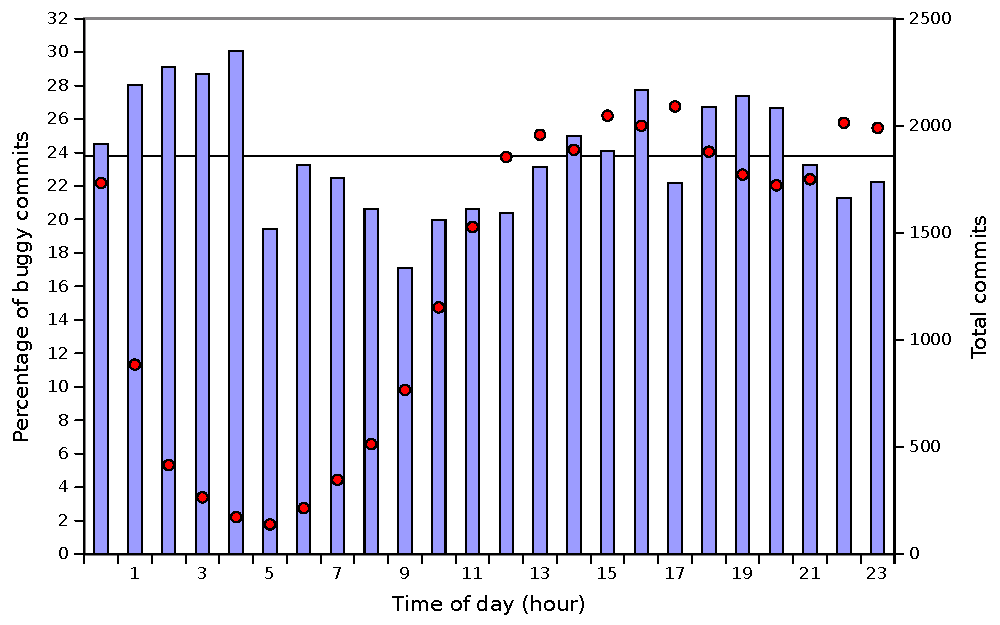
\includegraphics[width=\columnwidth]{postgresql-bugginess-hour.pdf}
\end{center}
\caption{PostgreSQL percentage of buggy commits (bars) and total number of commits (circles) versus time of day}
\label{fig-postgresql-bugginess-hour}
\end{figure}

%% \begin{figure}
%% \begin{center}
%% 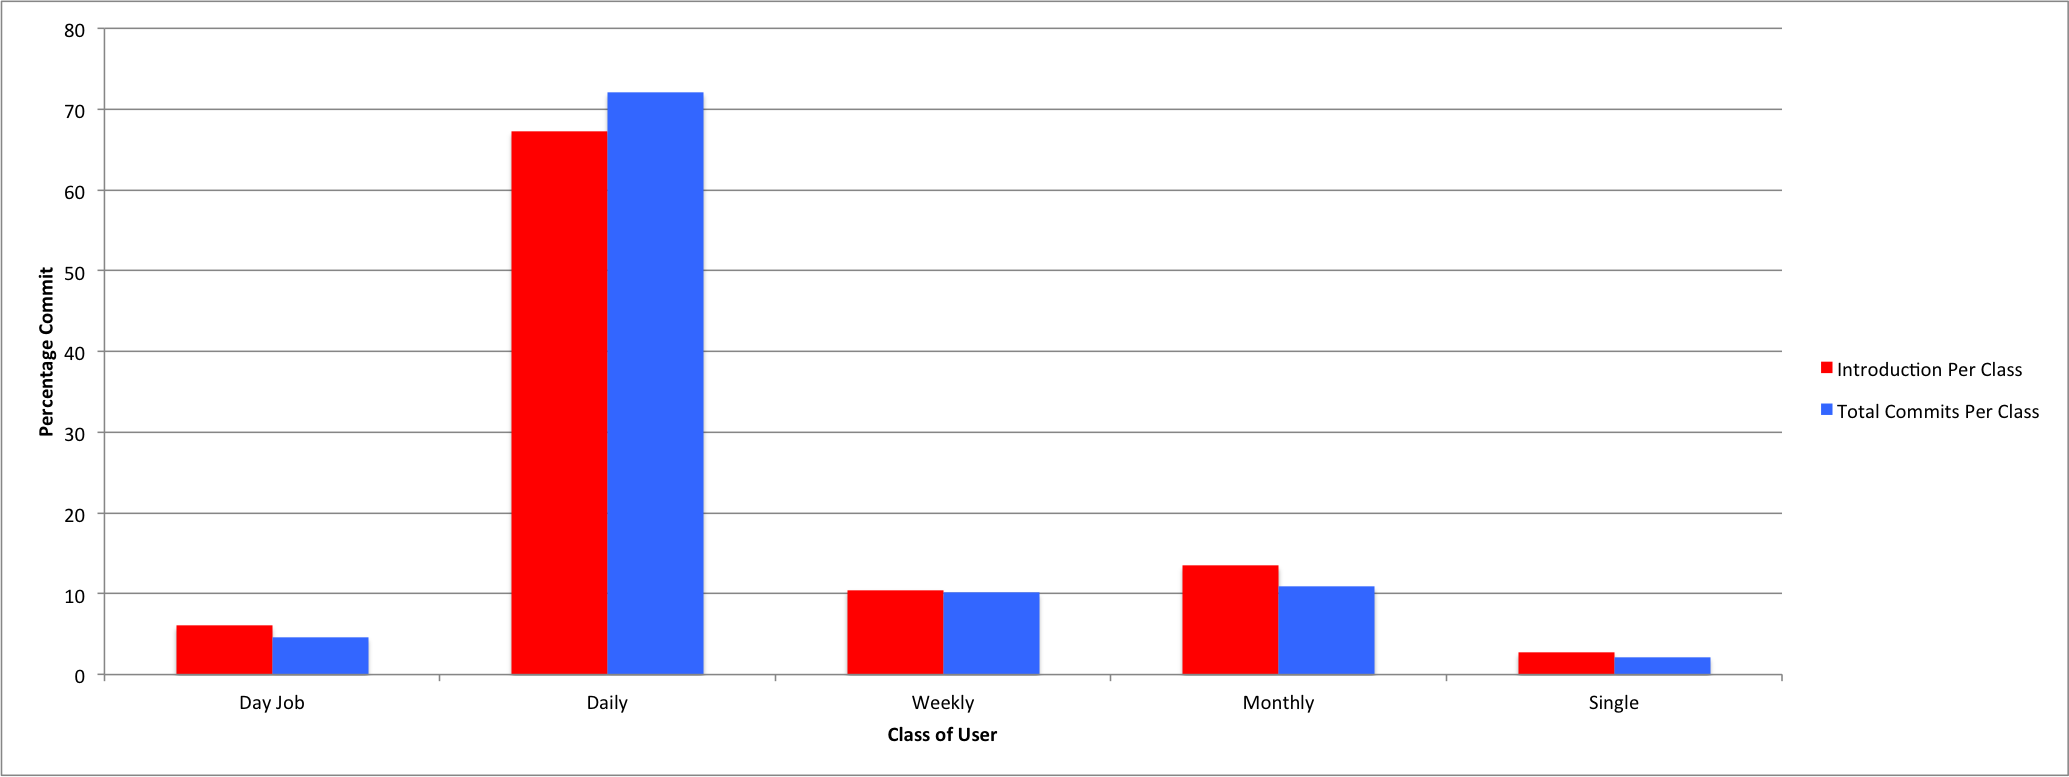
\includegraphics[width=0.45\textwidth]{linux_per_class.png}
%% \end{center}
%% \caption{Linux percentage of bug introductions and percentage of total commits per author classification}
%% \label{fig-linux-class}
%% \end{figure}

%% \begin{figure}
%% \begin{center}
%% 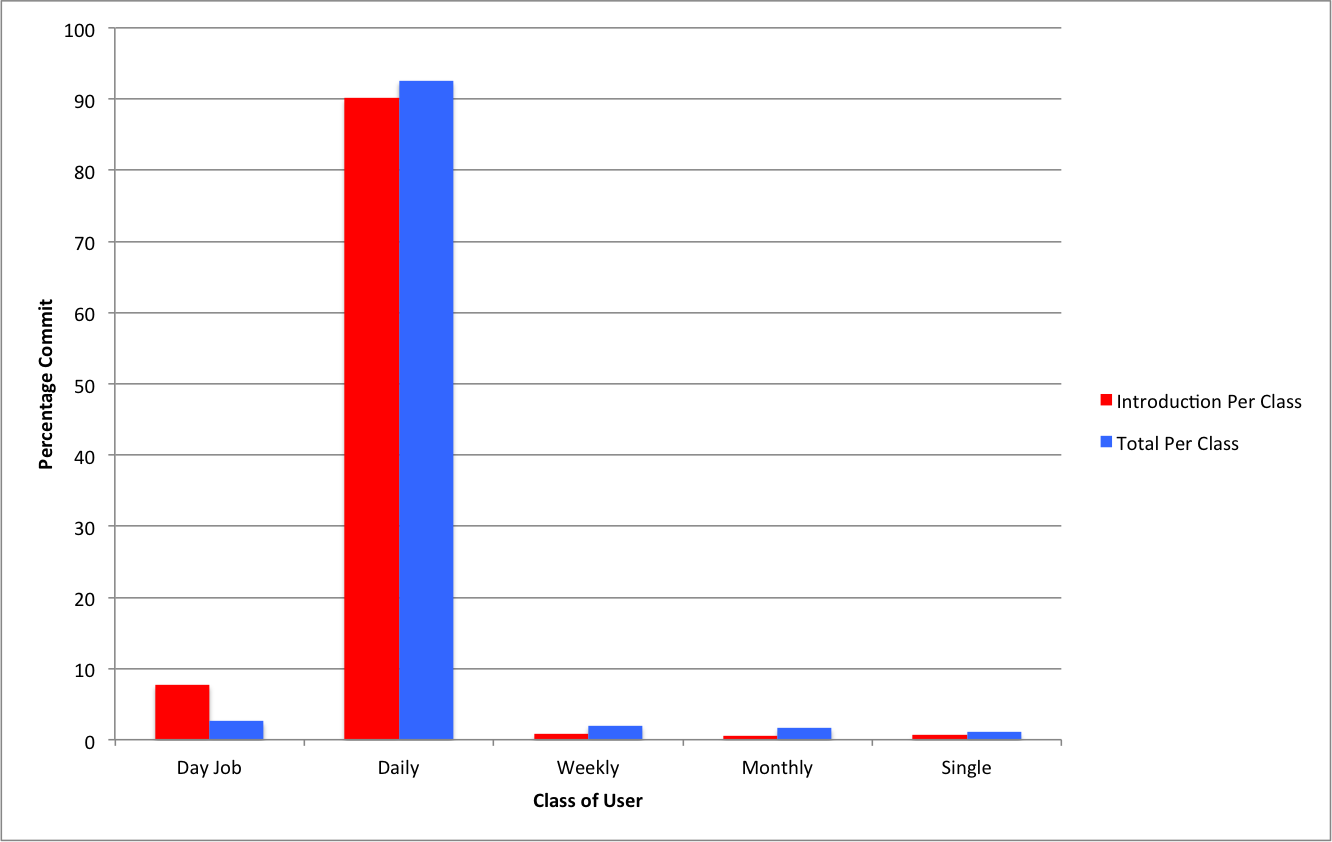
\includegraphics[width=0.45\textwidth]{firefox_per_class.png}
%% \end{center}
%% \caption{Firefox percentage of bug introductions and percentage of total commits per author classification}
%% \label{fig-firefox-class}
%% \end{figure}

\subsection{Developer Characteristics}
We next present our findings with respect to developer classification
and experience.  Developer classification summarizes the frequency of
a developer's contributions to a project, while developer experience
tracks how long a developer has contributed to a particular project.

\paragraph{Developer Frequency Classification} 
As we described in Section~\ref{sec:data}, one of the ways that we
classify developers is according to frequency, i.e. most-common
interval between consecutive commits---daily, weekly, monthly, other,
or single.  This information is only interesting for the Linux kernel, as the
almost all (28/34) of Postgres's committers are daily. We computed the
bugginess rates for each of these classes of developers and plot
author classification versus bug-introduction percentage in
Figure~\ref{fig-linux-bugginess-author-class}. The graph also presents
the number of authors in each class; the Linux kernel has 49 day job authors,
and 238 weekly and 288 monthly authors.

Our results show that the Linux kernel developers who commit changes daily, but
not as their day job, produce the smallest number of bug-introducing
commits, followed by the single-commit authors (whose patches would
presumably be simple or closely-reviewed). The day job, weekly, and
monthly committers all produce slightly more bug-introducing commits
than average.

A possible cause for the difference between day-job and daily
committers is that day-job developers might be required to make
changes by their employers, while the daily developers are motivated
purely by interest, and unlikely to be pressured to fix bugs on any
particular schedule.

\begin{figure}
\begin{center}
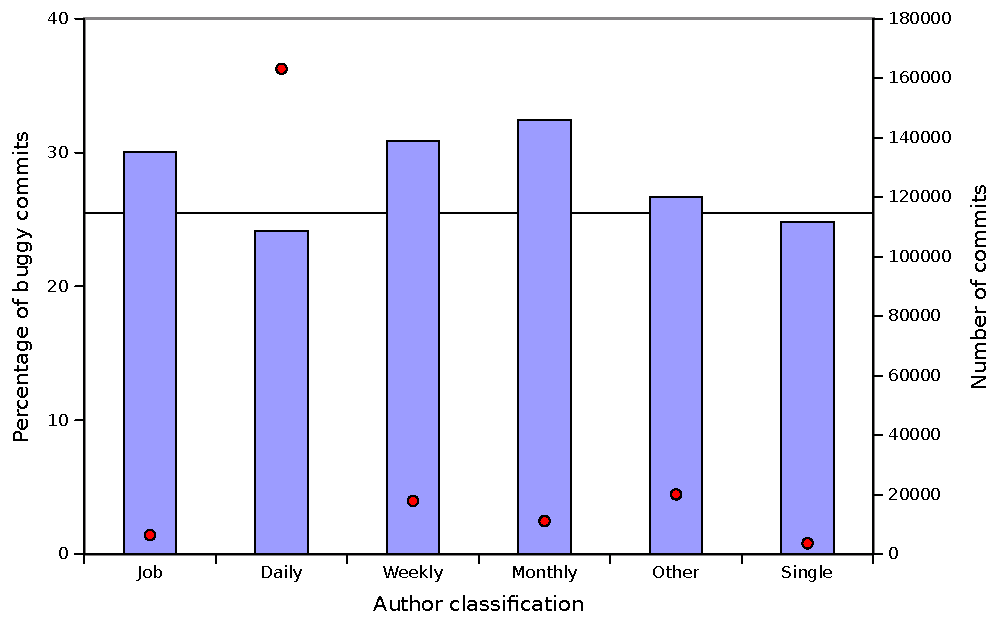
\includegraphics[width=\columnwidth]{linux-bugginess-author-class.pdf}
\end{center}
\caption{Linux percentage of buggy commits (bars) and number of authors (circles) versus author classification}
\label{fig-linux-bugginess-author-class}
\end{figure}

% we need to say what the two bars mean in the figure.

%% \begin{figure}
%% \begin{center}
%% 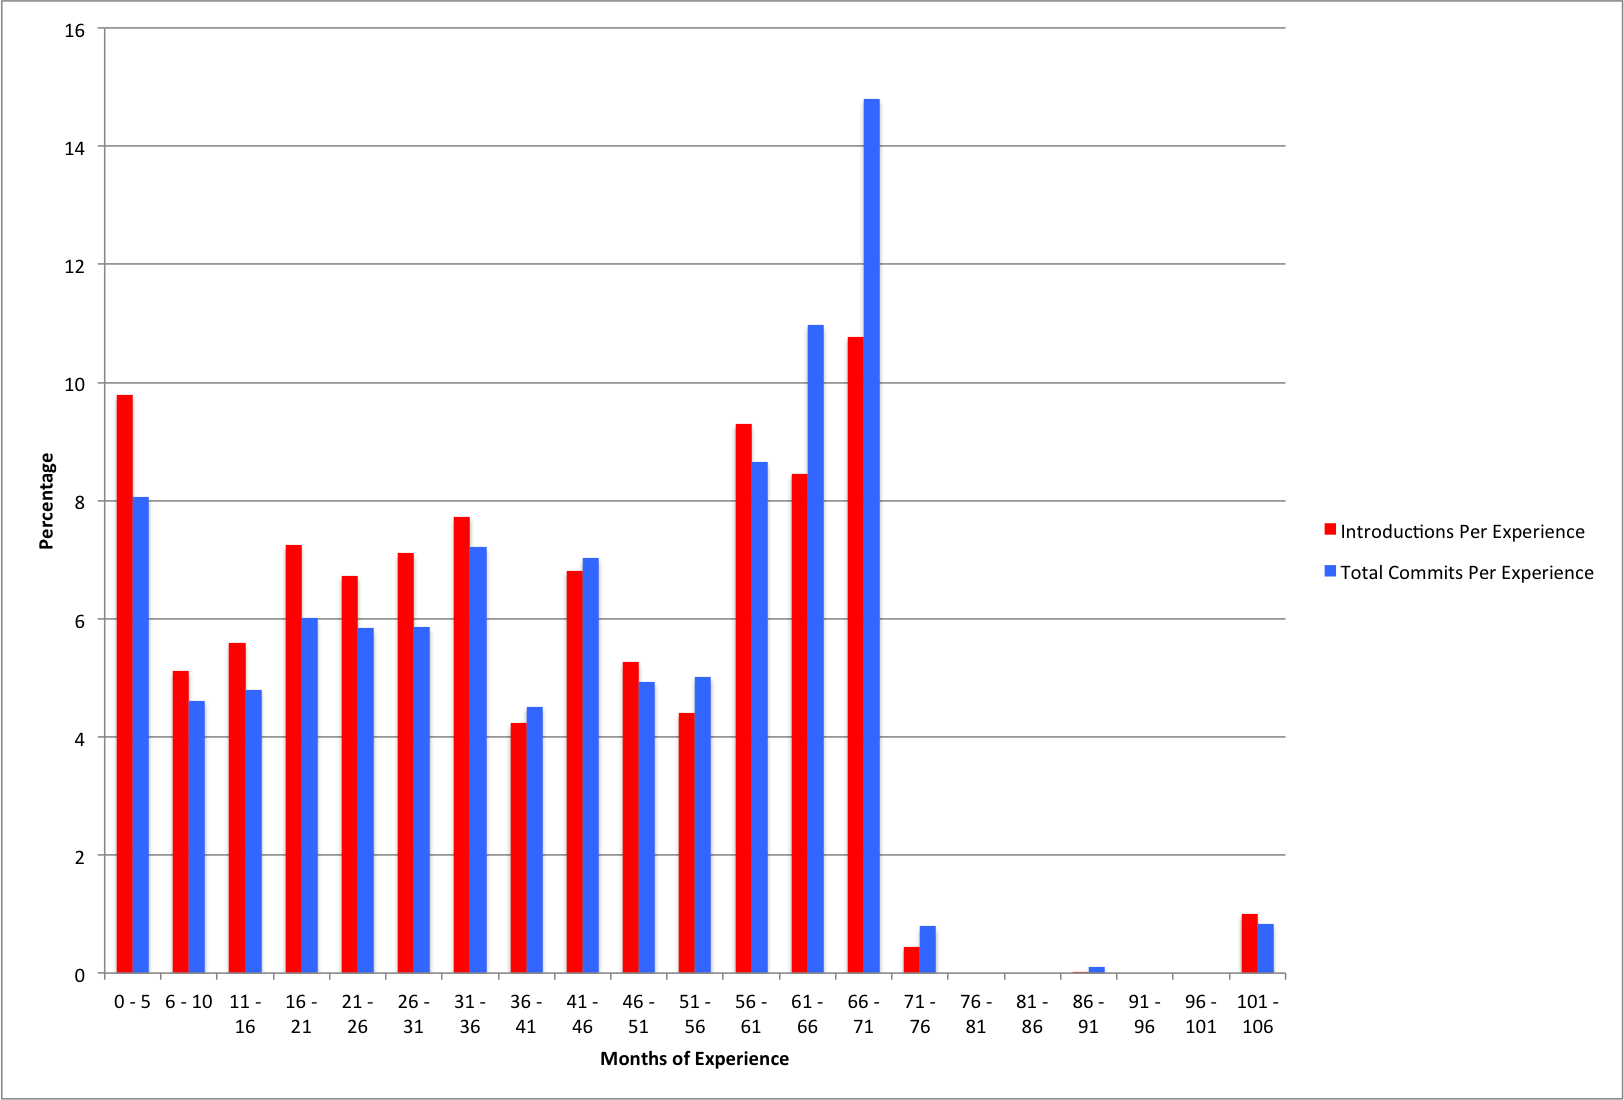
\includegraphics[width=0.45\textwidth]{linux_day_per_experience.png}
%% \end{center}
%% \caption{Linux percentage of bug introductions and percentage of total commits per author experience}
%% \label{fig-linux-experience}
%% \end{figure}

%% \begin{figure}
%% \begin{center}
%% 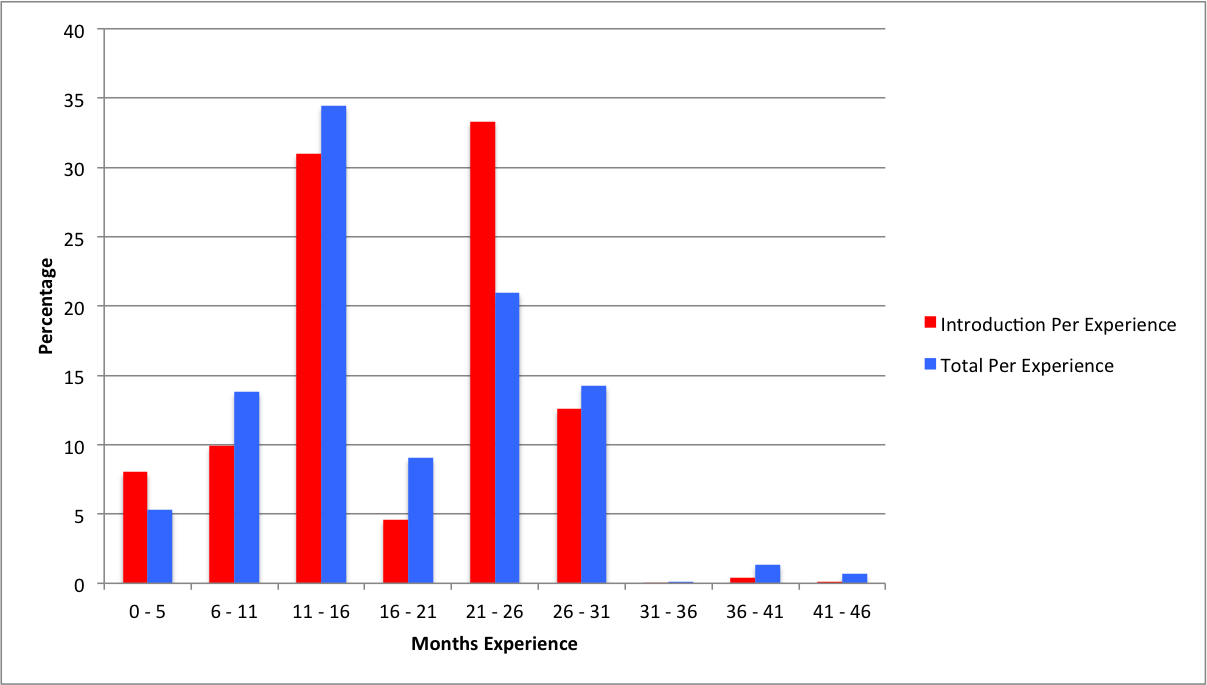
\includegraphics[width=0.45\textwidth]{firefox_day_per_experience.png}
%% \end{center}
%% \caption{Firefox percentage of bug introductions and percentage of total commits per author experience}
%% \label{fig-firefox-experience}
%% \end{figure}

\paragraph{Developer Experience Classification}
The final head-to-head comparison we performed is based on the amount
of experience per author. We divided them up into 6-month intervals. 
Our results from the Linux kernel and Firefox are shown in Figure
\ref{fig-linux-experience} and Figure \ref{fig-firefox-experience}
respectfully. For the Linux kernel authors with less than 2 years of experience
are more likely to commit a bug while after 2 years the likelihood
decreases. However the authors which committed throughout the history
of the project are more likely to commit a bug which may be because
they wrote the majority of the code. For Firefox, again the
developers with less than 6 months of experience are more likely to
commit a bug. The is a spike between 21 and 26 months as well. We
believe these results may not be accurate due to the possiblity of
our experience metric being crude and not representative of the 
actual experience with the project.

%% \begin{figure}
%% \begin{center}
%% 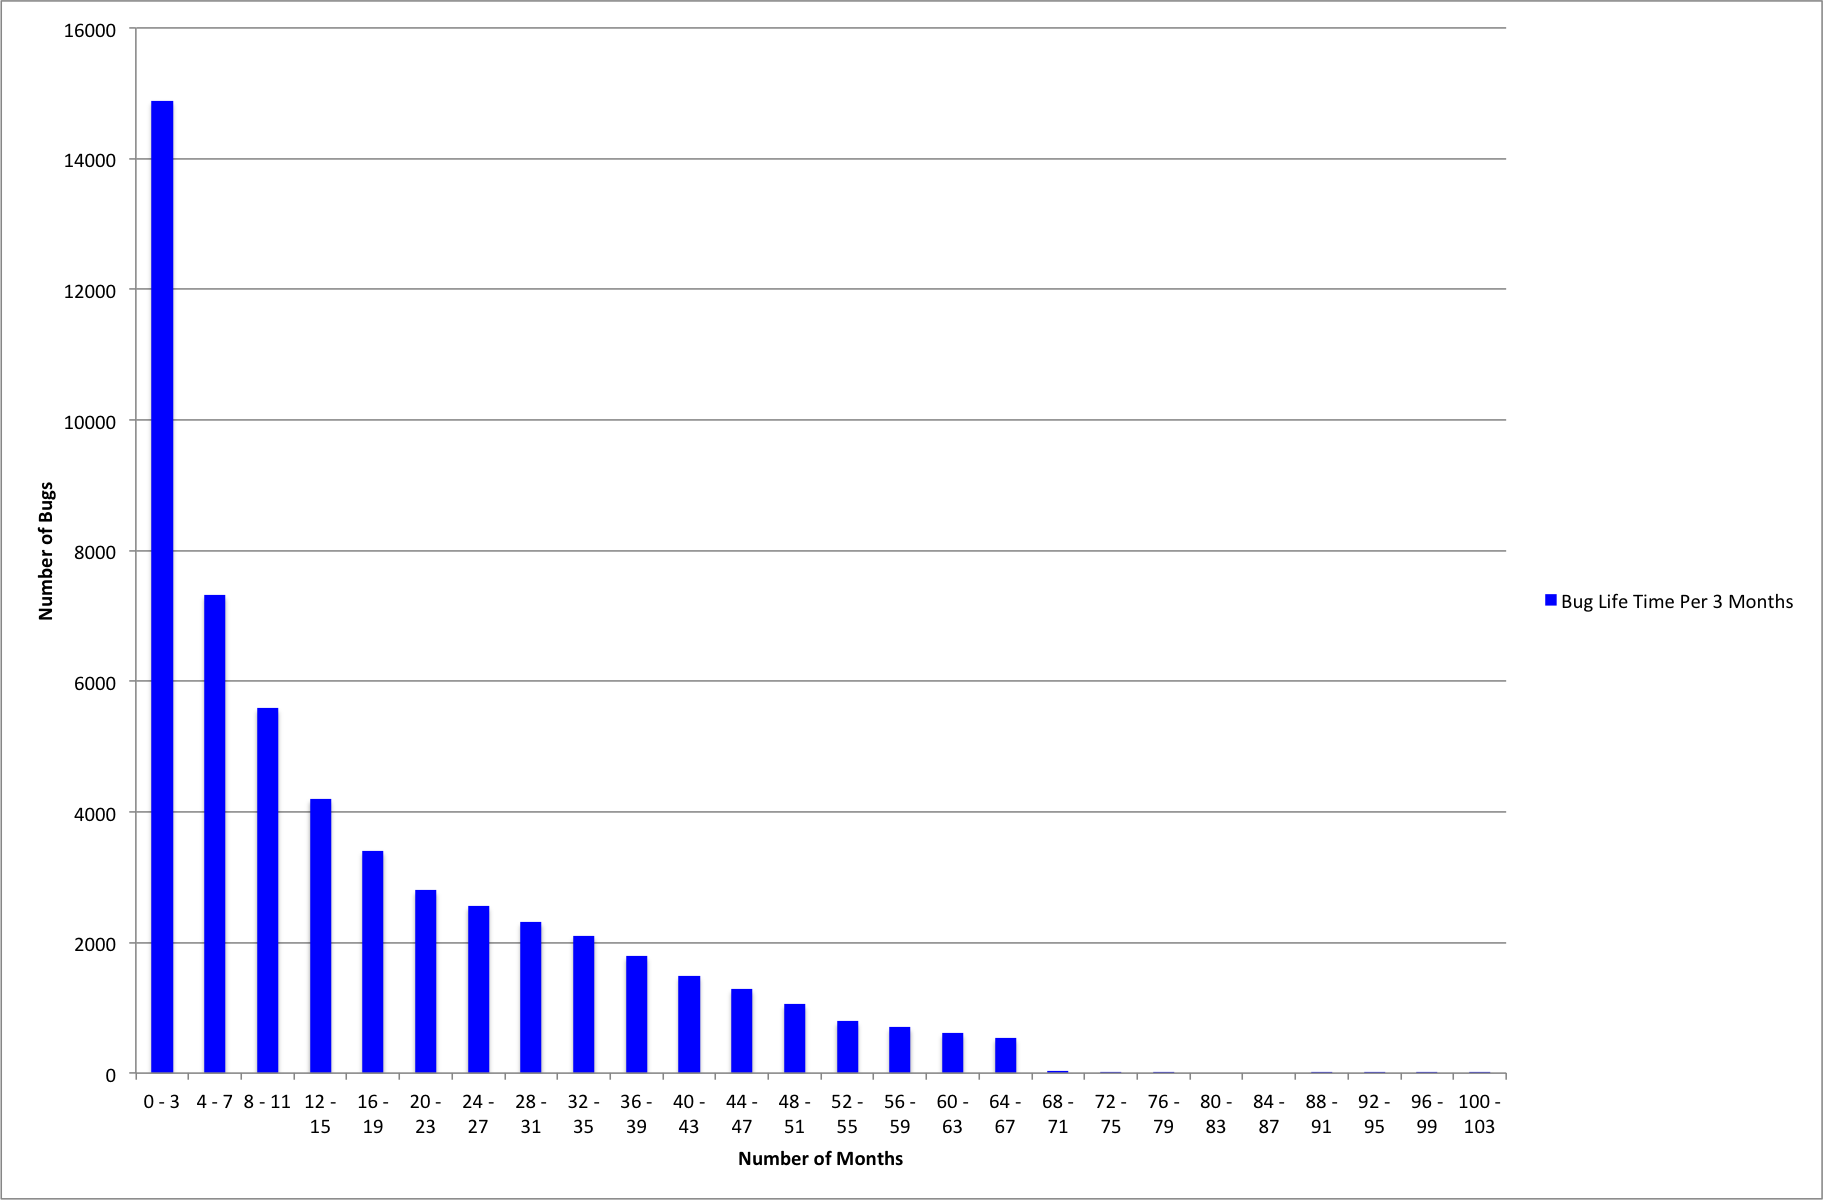
\includegraphics[width=0.45\textwidth]{linux_bug_life.png}
%% \end{center}
%% \caption{Linux number of bugs against bug lifetimes in months}
%% \label{fig-linux-buglife}
%% \end{figure}

%% \begin{figure}
%% \begin{center}
%% 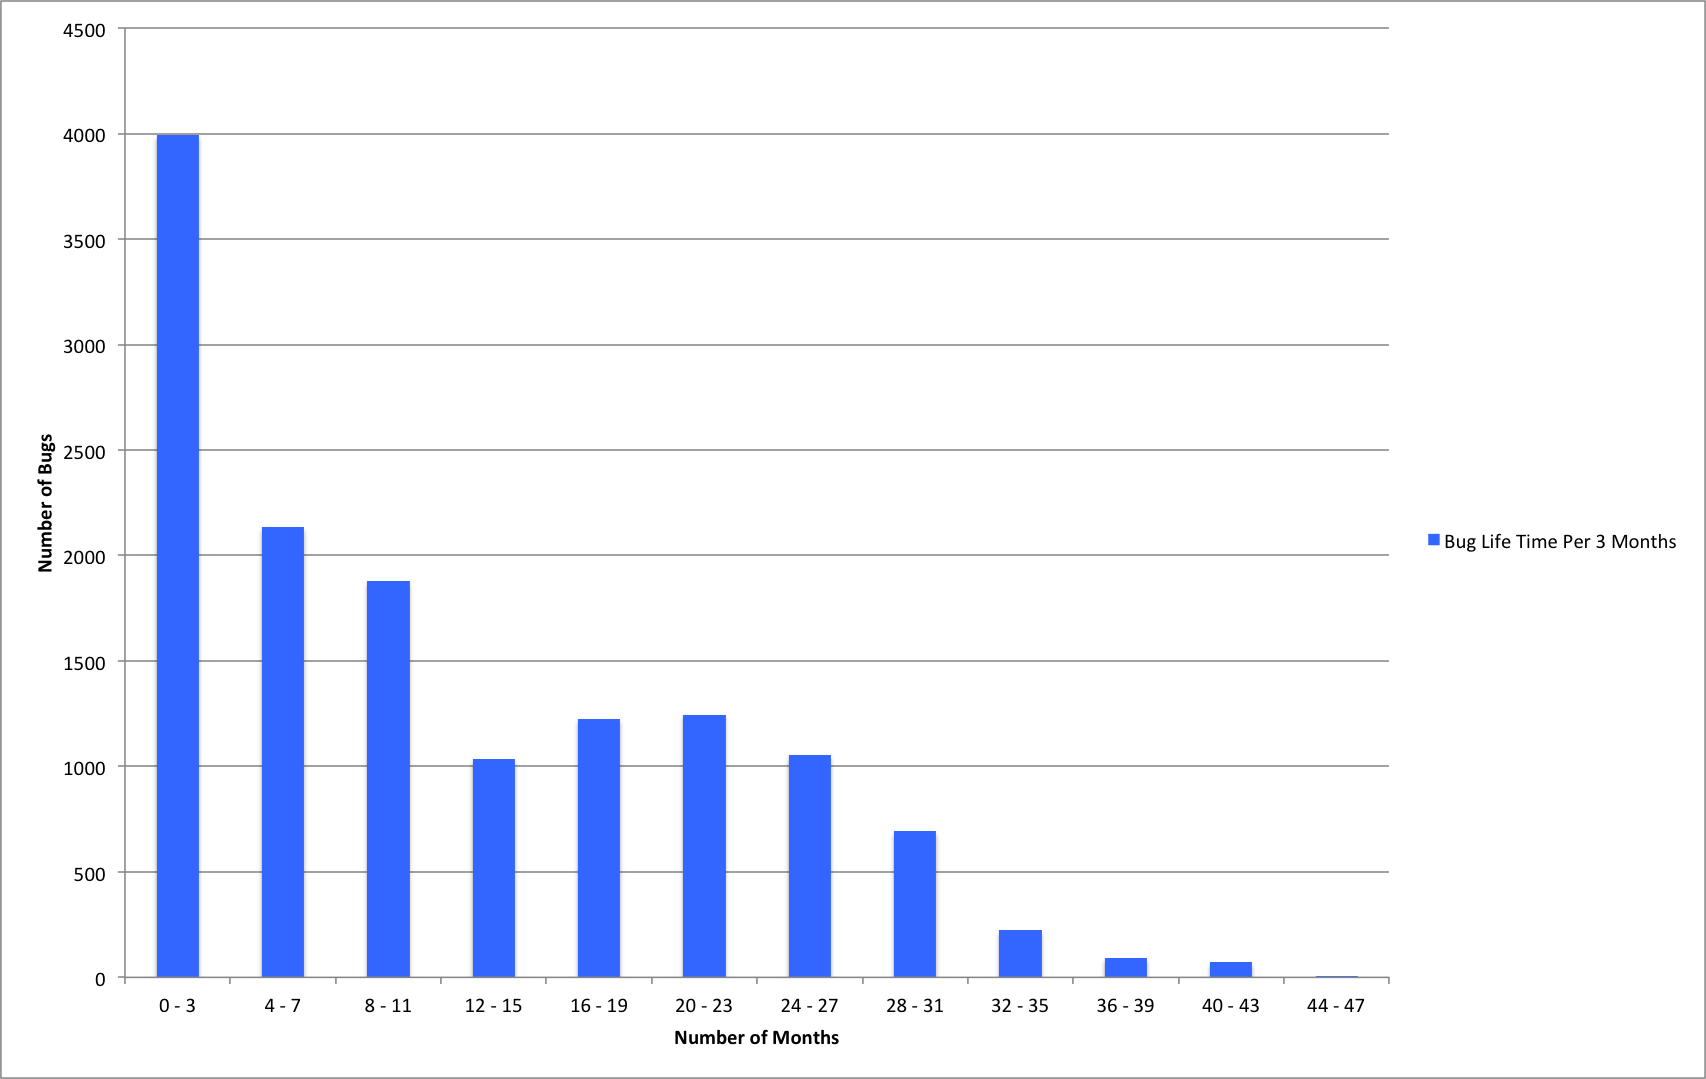
\includegraphics[width=0.45\textwidth]{firefox_bug_life.png}
%% \end{center}
%% \caption{Firefox number of bugs against bug lifetimes in months}
%% \label{fig-firefox-buglife}
%% \end{figure}

Finally we determined the bug lifetimes for both projects to contrast
them to previous work. We plotted the number of bugs for each lifetime
divided into 4 month intervals. The results for the Linux kernel are shown in
Figure \ref{fig-linux-buglife}, the average bug lifetime is 1.39
years. The results for Firefox are shown in Figure
\ref{fig-firefox-buglife}, with an average bug lifetime of 0.97
years. This shows a reduction in the average bug lifetime for the Linux kernel (in
2002 the average lifetime was 1.8 years). This indicates that
developers are improving as their development process becomes more
refined. We also see the average lifetime is lower for Firefox, this
may be due to the complexity of the software, size of the software or
the amount of users (the more users and complex, the more likely bugs will be
revealed).

%% \begin{figure}
%% \begin{center}
%% 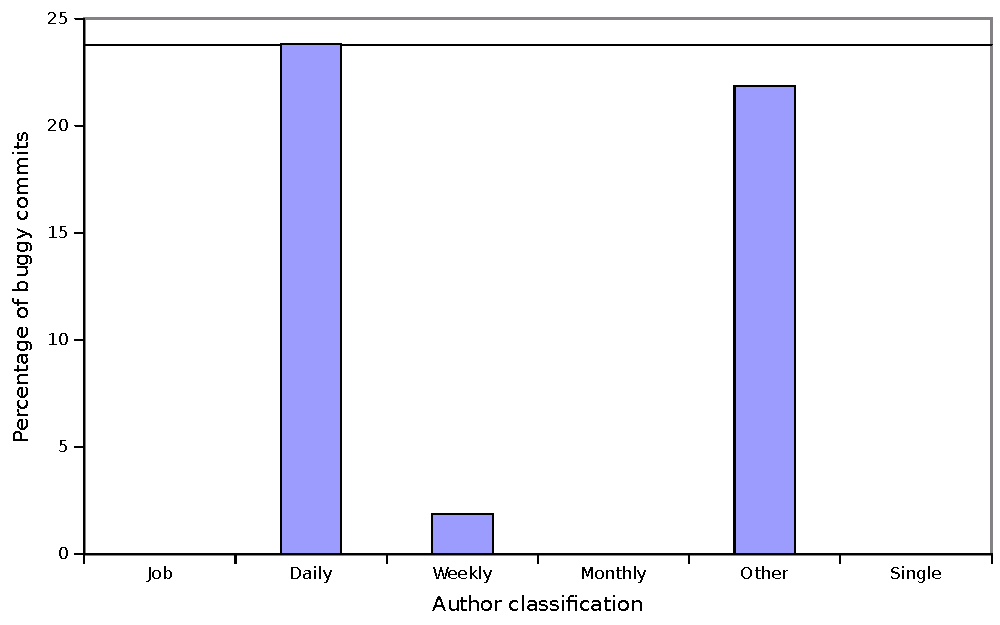
\includegraphics[width=0.45\textwidth]{postgresql-bugginess-author-class.pdf}
%% \end{center}
%% \caption{PostgreSQL percentage of buggy commits per author classification}
%% \label{fig-postgresql-bugginess-author-class}
%% \end{figure}

\begin{figure}
\begin{center}
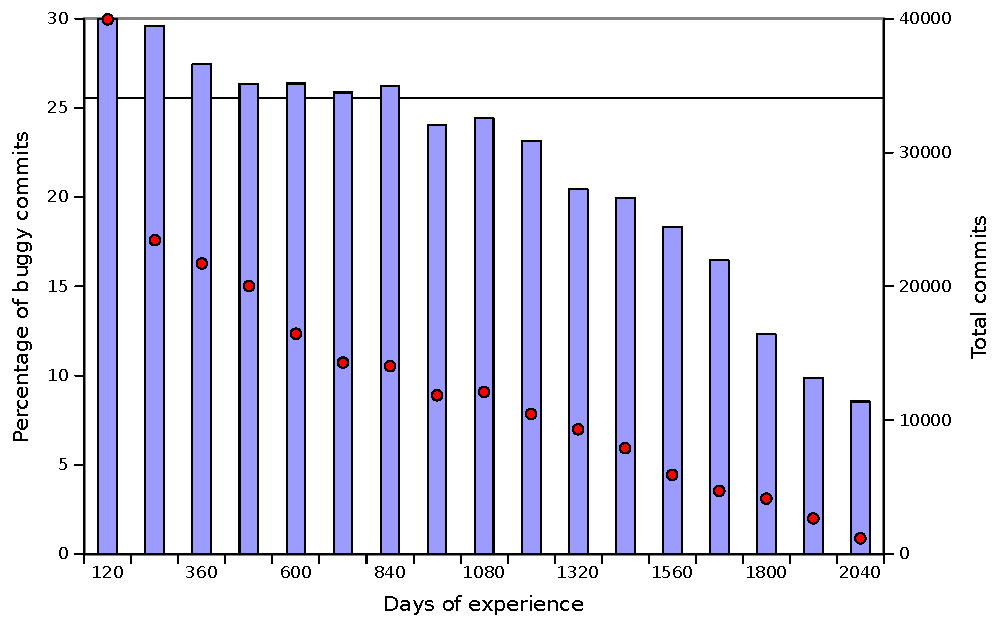
\includegraphics[width=\columnwidth]{linux-bugginess-experience.pdf}
\end{center}
\caption{The Linux kernel percentage of buggy commits per author experience}
\label{fig-linux-bugginess-experience}
\end{figure}

\begin{figure}
\begin{center}
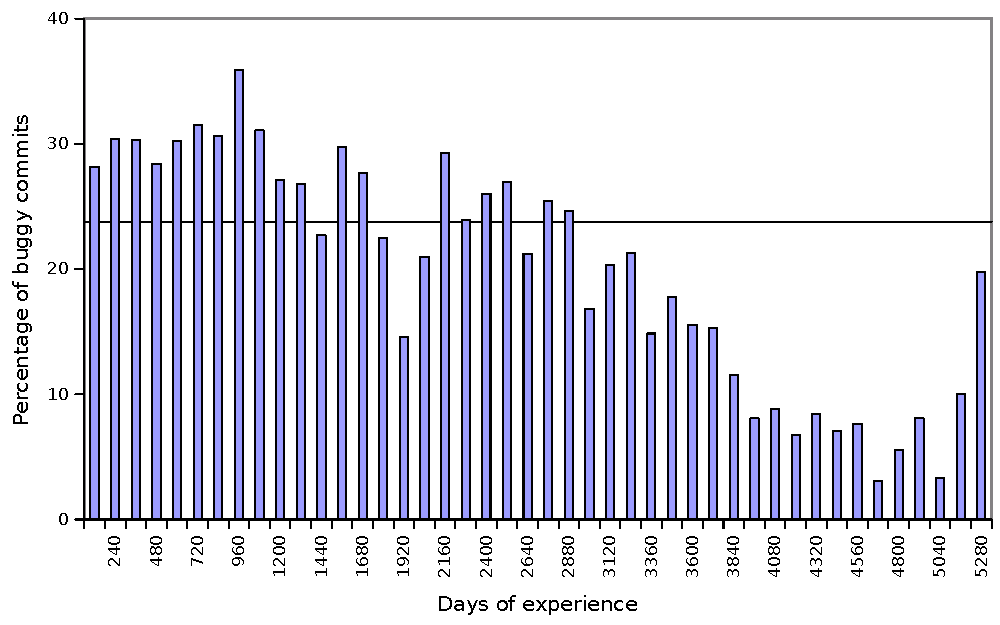
\includegraphics[width=\columnwidth]{postgresql-bugginess-experience.pdf}
\end{center}
\caption{PostgreSQL percentage of buggy commits per author experience}
\label{fig-postgresql-bugginess-experience}
\end{figure}


\begin{figure}
\begin{center}
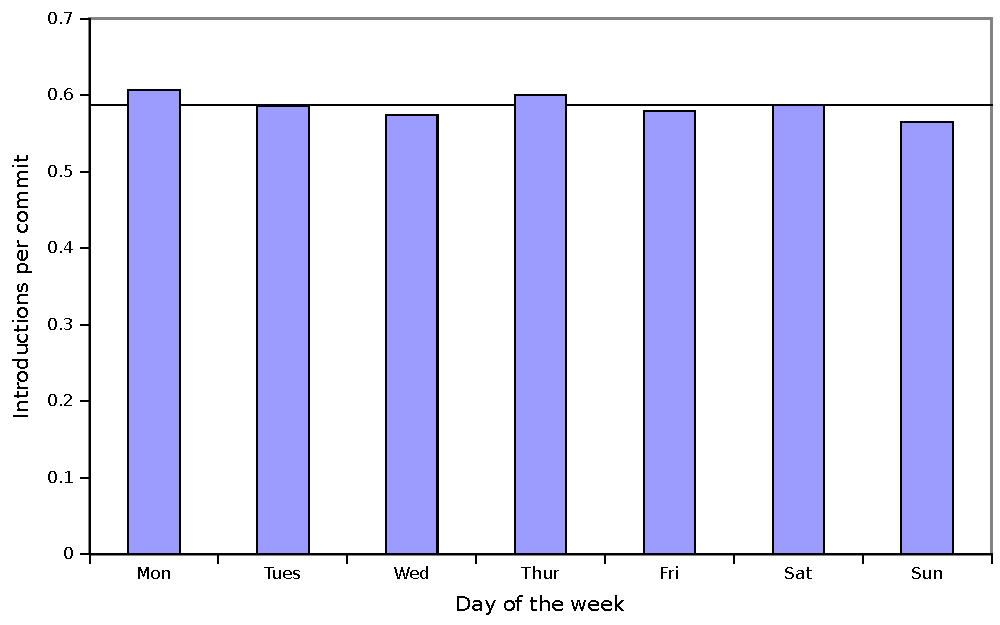
\includegraphics[width=\columnwidth]{linux-introductions-day.pdf}
\end{center}
\caption{The Linux kernel introductions per commit per day}
\label{fig-linux-introductions-day}
\end{figure}

\begin{figure}
\begin{center}
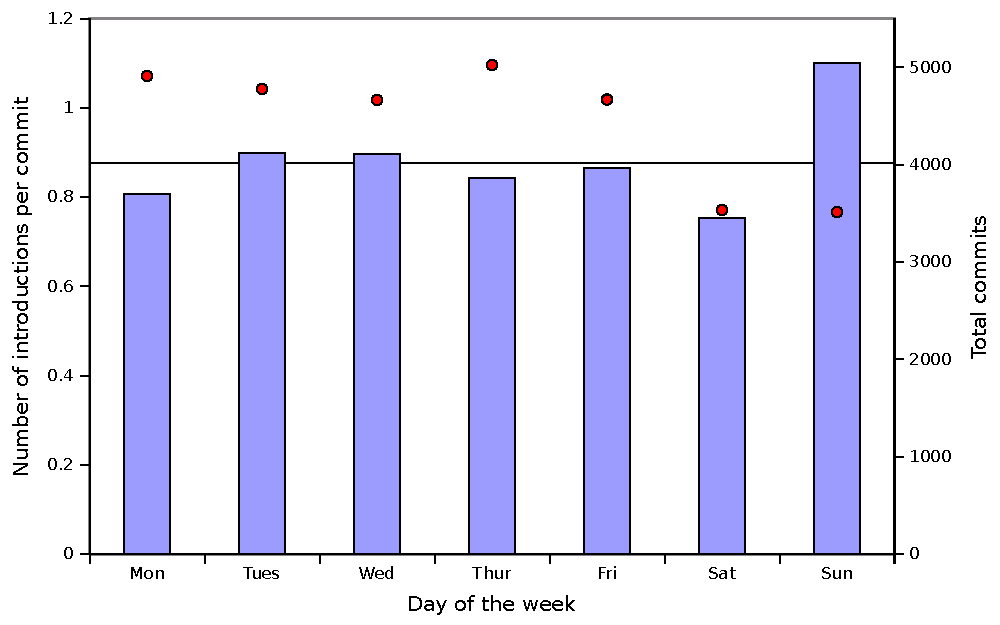
\includegraphics[width=\columnwidth]{postgresql-introductions-day.pdf}
\end{center}
\caption{PostgreSQL introductions per commit per day}
\label{fig-postgresql-introductions-day}
\end{figure}

\begin{figure}
\begin{center}
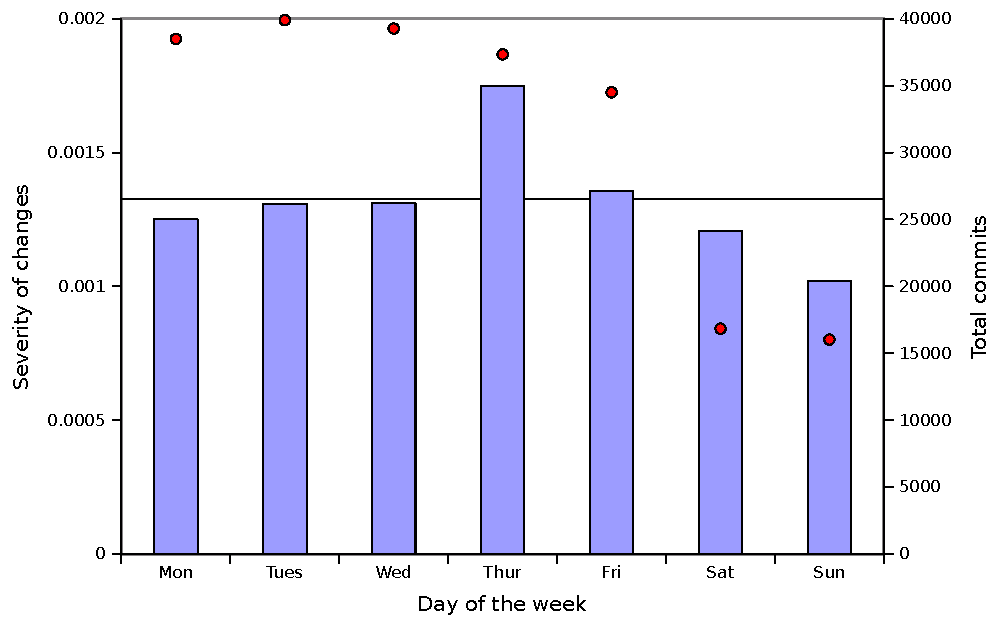
\includegraphics[width=\columnwidth]{linux-severity-day.pdf}
\end{center}
\caption{The Linux kernel severity of changes per day}
\label{fig-linux-severity-day}
\end{figure}

\begin{figure}
\begin{center}
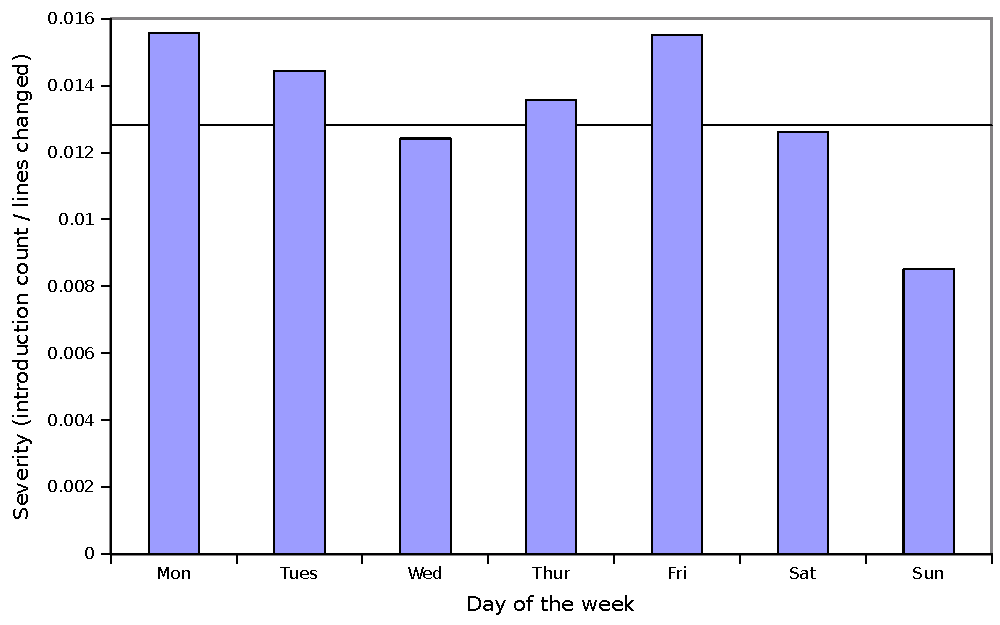
\includegraphics[width=\columnwidth]{postgresql-severity-day.pdf}
\end{center}
\caption{PostgreSQL severity of changes per day}
\label{fig-postgresql-severity-day}
\end{figure}

\begin{figure}
\begin{center}
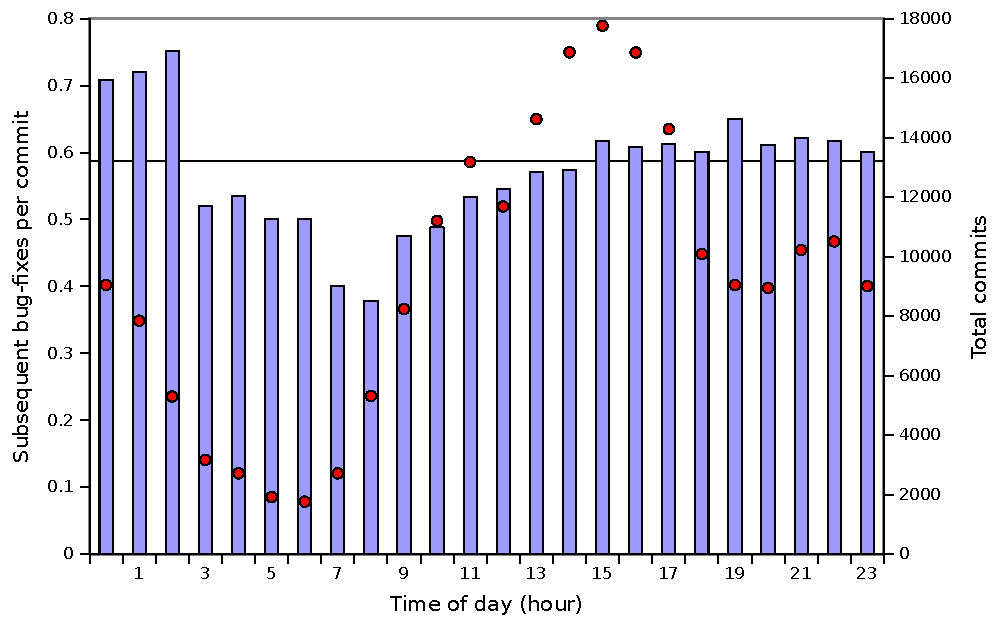
\includegraphics[width=\columnwidth]{linux-introductions-hour.pdf}
\end{center}
\caption{The Linux kernel introductions per commit per hour}
\label{fig-linux-introductions-hour}
\end{figure}

\begin{figure}
\begin{center}
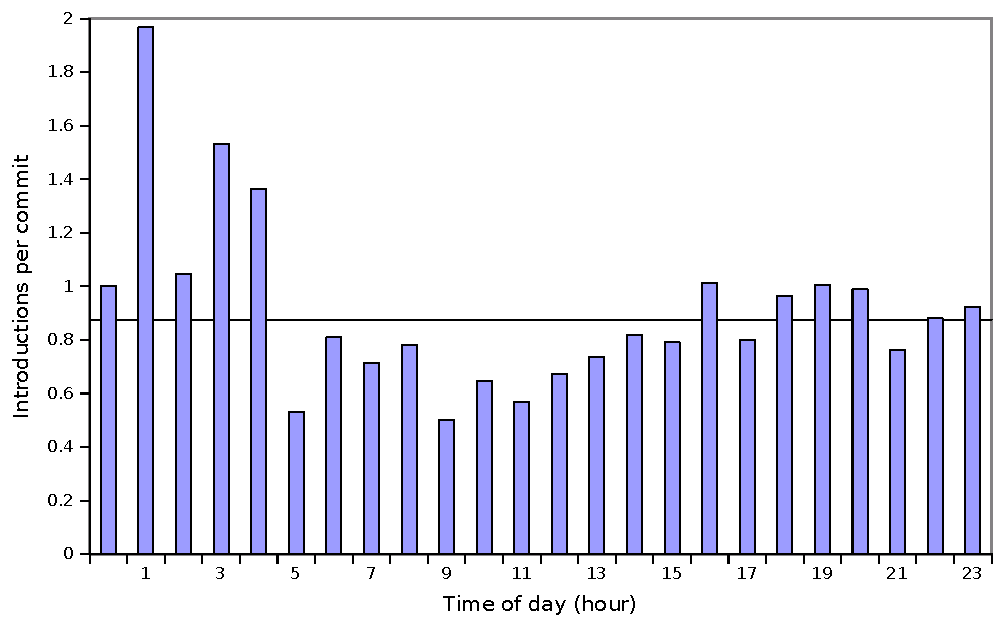
\includegraphics[width=\columnwidth]{postgresql-introductions-hour.pdf}
\end{center}
\caption{PostgreSQL introductions per commit per hour}
\label{fig-postgresql-introductions-hour}
\end{figure}

\begin{figure}
\begin{center}
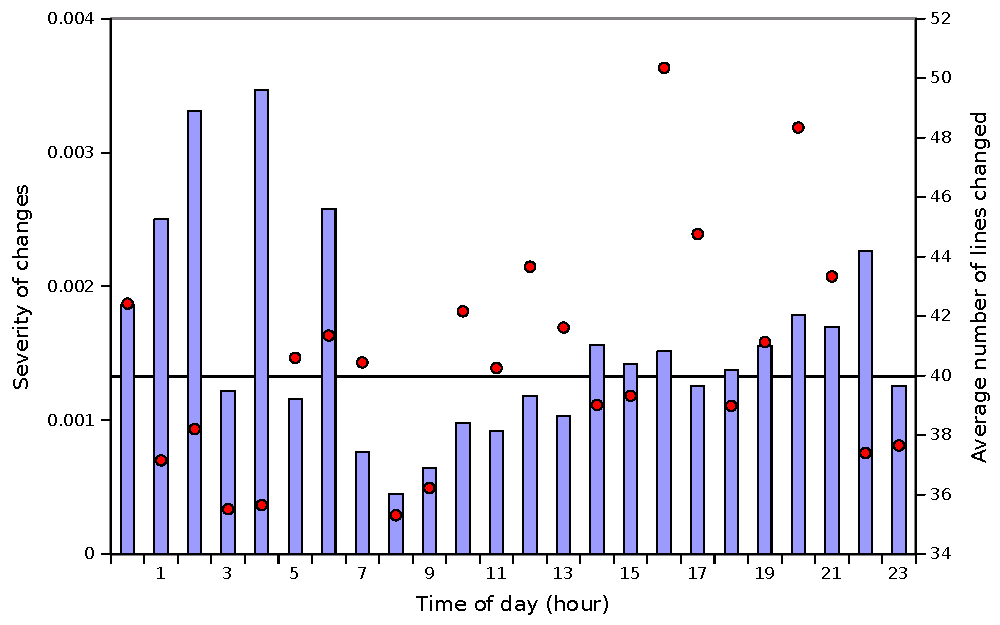
\includegraphics[width=\columnwidth]{linux-severity-hour.pdf}
\end{center}
\caption{The Linux kernel severity of changes per hour}
\label{fig-linux-severity-hour}
\end{figure}

\begin{figure}
\begin{center}
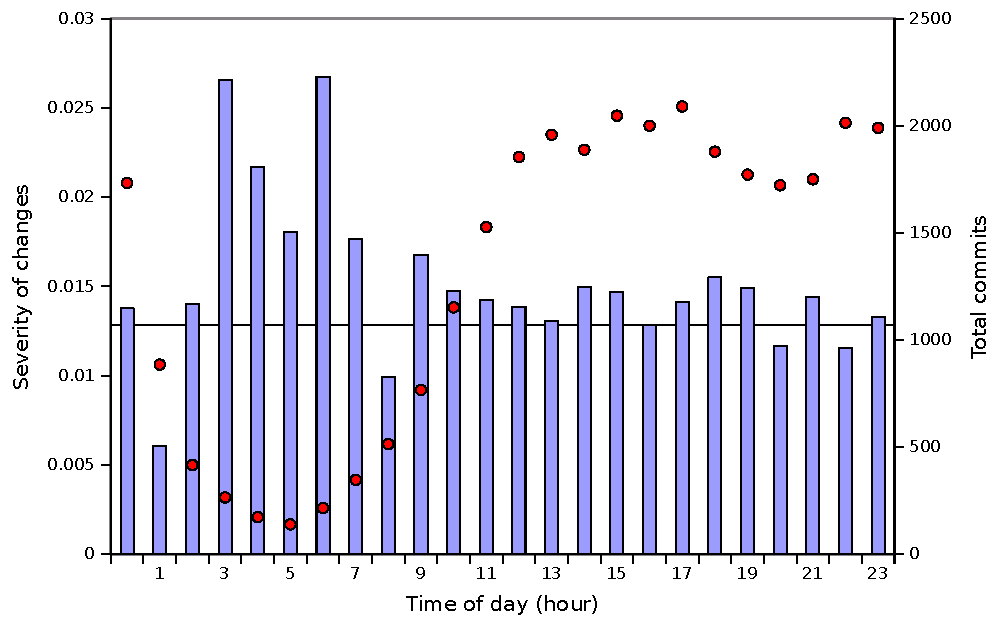
\includegraphics[width=\columnwidth]{postgresql-severity-hour.pdf}
\end{center}
\caption{PostgreSQL severity of changes per hour}
\label{fig-postgresql-severity-hour}
\end{figure}

\begin{figure}
\begin{center}
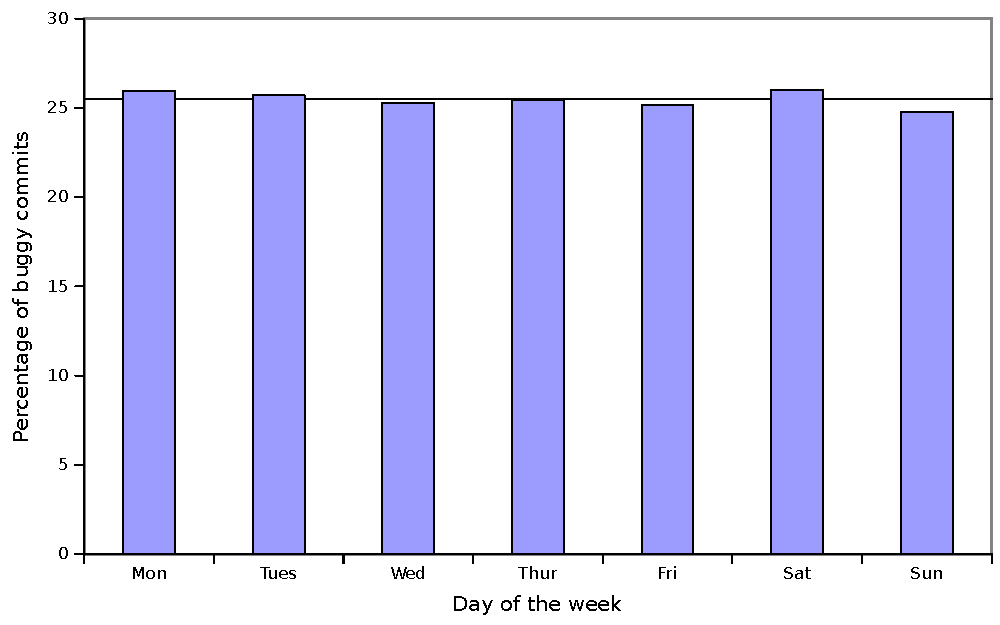
\includegraphics[width=\columnwidth]{linux-bugginess-day.pdf}
\end{center}
\caption{The Linux kernel percentage of buggy commits per day}
\label{fig-linux-bugginess-day}
\end{figure}

\begin{figure}
\begin{center}
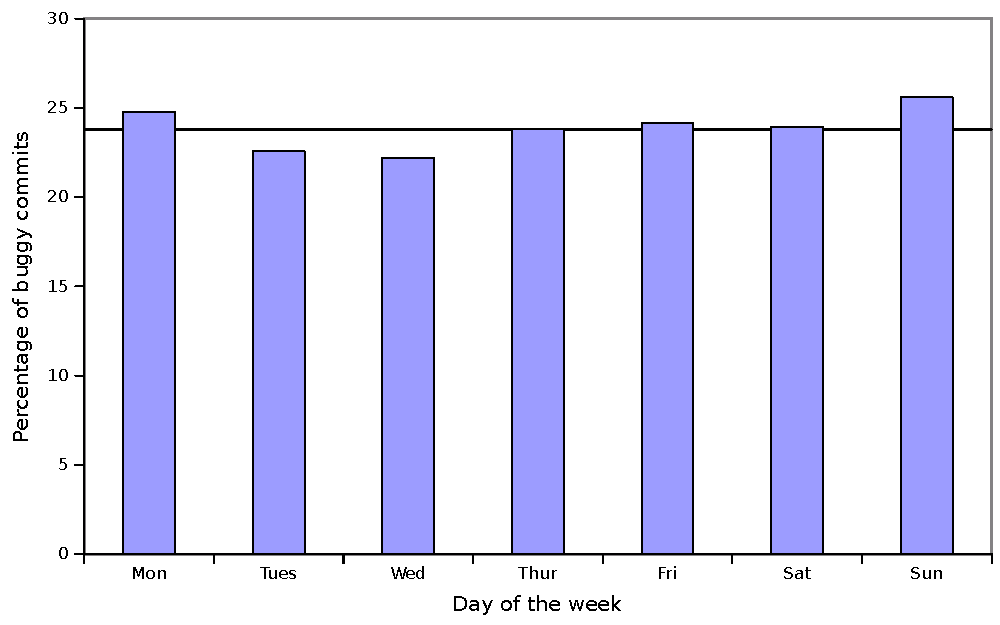
\includegraphics[width=\columnwidth]{postgresql-bugginess-day.pdf}
\end{center}
\caption{PostgreSQL percentage of buggy commits per day}
\label{fig-postgresql-bugginess-day}
\end{figure}

\subsection{Day-of-week Results} Having determined our false positive rate, 
we continue by presenting the results of our analysis.  First, we
determine if the day of the week has any impact on the likelihood of
producing bugs. For the following graphs, the percentage of
introduction commits indicates the amount of commits which are bug
introductions, as a propostion of the total number of
commits. Figure~\ref{fig-linux-bugginess-day} presents our results for
the Linux kernel. We see that Saturday is the worst day, followed by Thursday,
while Monday has the fewest percentage of bug introductions. The
results for Firefox are shown in Figure~\ref{fig-postgresql-bugginess-day} and
agree with Thursday being one of the worst days, while Monday is the
best day for committing changes which do not introduce bugs. A
possible explanation is that developers rest over the weekend and have
ample time to think about the problem before coding a solution on
Monday, when they know exactly what to do. Per-day bugginess may also
be correlated with the size of the change, which we plan to investigate
later, as an addition to our technique.

\subsection{Comment-only Commits}
We noticed that a surprisingly large number of bug-fixing commits only 
changed comments in the source code.

%% We also noted that approximately 7.7\% of the bug fixes for Linux were
%% purely for comments, indicating that developers spend a non-trivial
%% amount of time on comments. For Linux, approximately 51\% of the
%% changes do not include additions. We therefore manually checked (a
%% subsample of) the 49\% more difficult cases to evaluate the
%% effectiveness of our heuristic for additions.

\subsection{Validation} 
To validate our results, we estimated the precision and recall of our
technique for identifying bug-fixing commits on both projects.  As our
algorithm for identifying the associated bug-introducing commits was a
straightforward application of git blame, we did not systematically
verify its performance. (A brief manual inspection of bug-introducing
commits looked correct.) For both projects, we randomly sampled 50 bugs
from each of the population of commits that we identified to be
bug-introducing commits BI (to evaluate precision) and commits that we
identified to be non-bug-introducing commits $\neg$ BI (to evaluate recall).
Tables~\ref{tab:pr-raw} and~\ref{tab:pr-adj} summarize our precision and
recall findings.

We evaluated the precision---that is, the proportion of identified
bug-fixing commits which do indeed fix bugs---and found that, for
the Linux kernel, 43 of the 50 bugs that we automatically identified as
bug-fixing commits did indeed fix bugs, while 7 did not; for Postgres,
42 of 50 identified fixes were indeed fixes.  Some of the
cases included: 1) a commit message which fixed a merge commit was
classified as a fix; 2) apparently garbled commit messages which
included the keyword ``fix'' for no good reason; 3) changes which were
reverted (in the alleged ``fix'') but then re-added in a later
version; 4) poor uses of version control systems which included many
different changes in a single commit, including a fix as a small part 
of the commit; and 5) refactoring changes, which moved or renamed
functions---these could arguably be considered to be fixes to a buggy
initial design.

To evaluate the recall of our technique, we sampled 50
non-bug-introducing commits from both the Linux kernel and
Postgres. Table~\ref{tab:pr-raw} presents the raw data. However, the
raw data must be adjusted before it will indicate the recall, because
the recall must be calculated as a proportion of commits over the
entire population of commits. We therefore adjusted our data to the
numbers shown in Table~\ref{tab:pr-adj}.

% WRITE MORE TEXT HERE.
% make this more clear

\begin{table}
\begin{center}
\begin{tabular}{rrr}
Linux & T & F \\
BI & 43 & 7 \\
$\neg$ BI & 6 & 44 \\
\end{tabular} \begin{tabular}{rrr} Postgres & T & F \\
BI & 42 & 8 \\
$\neg$ BI & 3 & 47
\end{tabular}
\end{center}
\caption{\label{tab:pr-raw}Raw results for precision and recall.}
\begin{center}
\begin{tabular}{rrr}
Linux & T & F \\
BI & 43 & 7 \\
$\neg$ BI & 23 & 172 \\
\end{tabular} \begin{tabular}{rrr} Postgres & T & F \\
BI & 42 & 8 \\
$\neg$ BI & 21 & 332
\end{tabular}
\end{center}
\caption{\label{tab:pr-adj}Adjusted results for precision and recall.}
\end{table}



%\input{discussion}
%\section{Related Work}
\label{sec-related}

We survey work related to our study of factors affecting bugginess (namely,
day-of-week); prior work on empirical studies of commits; studies of bugginess
in distributed software development; and empirical studies on bug lifetime.

\paragraph{Day of Week of Commits}

The most closely related work to ours, \'Sliwerski et
al~\cite{sliwerski-msr-2005}, studied the day of the week of commits for two
totally different projects, Eclipse and Mozilla, and found that the commits on
Fridays are buggiest. This paper differs from the work of \'Sliwerski et al in
the following three key aspects. Firstly, we investigated how the commits' time
of day correlates with the bugginess of commits, which has not been studied
before, to the best of our knowledge. Secondly, we studied developer
characteristics, including correlations between commit bugginess and developers'
activity levels, as well as developers' experience, which the previous work did
not study. Finally, we used different data collection techniques. Specifically,
we did not rely on the link between a commit and a bug report to extract
bug-fixing commits, which enabled us to study software for which such links are
not maintained or not well maintained by the developers. For example, we found
that only 2.3\% of the Linux kernel's bug-fixing commits are linked to a bug
report, by manually examining a random sample of our bug-fixing commits. While
using links between bug reports and bug commits may increase the precision of
extracting bug-fixing commits, our results demonstrate that high precision can
be obtained without using such links: the precision of our bug-fixing commit
extraction techniques are \linuxP for the Linux kernel and \postP for
PostgreSQL.

%% Note: 2.3\% (1/43)

\paragraph{Empirical Studies on Commits}

Many empirical studies have been conducted to understand and leverage different
aspects of
commits~\cite{hattori2008nature,largeCommits,commitTextualClassification,
  smallCommits05, Swanson76}, which studied the distributions of commit sizes
and how commit sizes correlate with other metrics such as different development
activities, commit classifications, etc.

%% Edit: For example, ... sounds awkward.
Hindle et al~\cite{largeCommits} classified commits into different categories,
one of which is non-functional commits (e.g., modification of comments,
documentation, etc.).  Our study differs from~\cite{largeCommits} in that we
specifically investigated comment-fixing commits. For example, a refactoring
commit would be considered to be a non-functional commit by the previous study,
but not a comment-fixing commit in this paper. iComment~\cite{iComment} only
showed that FreeBSD contains many comment-fixing commits; it is not a
comprehensive study on comment-fixing commits.  We estimate that about 1,200 and
130 commits (Section~\ref{sec-comment-only}) in the Linux kernel and PostgreSQL,
respectively, only fix comments, and do not modify the code, showing that
developers spent time maintaining the correctness of comments.

\paragraph{Distributed Software Development and Code Quality}

Several previous studies sought to understand how distributed software
development affects code quality~\cite{distributed09, organizational08,
  global06} in open source and commercial software. While the two pieces of
software we studied are open-source and developed in a distributed fashion, the
goal of this paper is different from these prior studies---we aim to understand
the correlation between code bugginess and social characteristics of commits,
e.g., commits' time of day, commits' day of week, developers' experience, and
developers' activity frequencies, etc.

\paragraph{Bug Lifetime}

Engler et al~\cite{deviant} examined the bug lifetime of the Linux kernel in
2001. Our study on the bug lifetime complements theirs by analyzing recent
commits to the Linux kernel from 2005-2010.  Kim and Whitehead~\cite{2006-long}
examined the bug lifetimes in PostgreSQL.  Neither of the two previous studies
investigated social characteristics such as commit time and author experience.

%% % Commit classification, cited above
%% \paragraph{On the Nature of Commits}

%% This paper studies the nature of commits in two dimensions: define the size of
%% commits in terms of number of files, and classify commits based on the content
%% of their comments \cite{hattori2008nature}. The authors investigated the
%% distribution of commits according to the number of files, and their results show
%% that the majority of commits contain a large number of files. The authors also
%% developed a classification system for commits according to development and
%% maintenance activities based on the content of their commits, a system that is
%% more suitable for open source projects. Some of the major findings made by the
%% authors include: the majority of the commits are not related to the development
%% activities, corrective actions generate more tiny commits, and development
%% activities are spread among all sizes of commits.

%% % Cited it in methods (about git blame)
%% \paragraph{Automatic identification of bug-introducing changes}

%% The authors try to automate the process of finding bug-introducing changes,
%% which would remove the manual work associated with going through bug reports or
%% commit logs to collect this type of information. They use the SZZ algorithm,
%% which traces from the location of the fix where the bug was introduced, and as
%% such extract the time \cite{2006-automatic}. The weakness with this algorithm is
%% that sometimes it makes false detections because not all modifications are
%% fixes, and a moderate improvement from using just SZZ is the use of annotation
%% graphs. Another improvement was ignoring format changes, which reduce a large
%% number of false positives. This paper has inspired the approach we used for
%% automating the process of identifying bug-introducing changes, which was key for
%% collecting a large pool of data.

%% % Not that related
%% \paragraph{How long did it take to fix bugs?}

%% In this paper the author try to measure software quality as a function of the
%% number of bugs. The authors examine the bug fix time of files in two open source
%% software: ArgoUML and PostgreSQL, and tackle this issue by identifying when bugs
%% are introduced and when the bugs are fixed \cite{2006-long}. The argument is
%% files with the greatest bug-fix times, whose bug counts are greater than
%% average, may need more attention to determine why bug fixes take such a long
%% time – potentially indicating the need for code refactoring to achieve faster
%% bug fixes in the future. The authors first extracted change histories of the two
%% projects, ArgoUML and PostgreSQL, using the Kenyon infrastructure. To identify a
%% bug-fix, they searched for keywords such as fixed or bugs and they also searched
%% for references to bug reports. They then applied the identified bug-introducing
%% changes by applying the fix-inducing change identification algorithms described
%% in the paper “When do changes induce fixes?” which I mentioned earlier.  This
%% work is of course relevant because it gives us a methodology for extracting
%% bug-fix times.

%% % Replaced by their later work zimmermann-promise-2007, cited in intro
%% \paragraph{If your bug database could talk}

%% This is another relevant work, where the authors perform experiments that
%% demonstrate how to relate developer, code, and process to defects in the
%% code. This work tries to understand why some programs are more failure-prone
%% than others.  To answer this question, we have to know which programs are more
%% failure-prone than others – to search for properties of the programs or its
%% development process that commonly correlate with defect density. The authors try
%% to answer questions like “can one predict failure-proneness from metrics like
%% code complexity?”, “what does a high number of bugs found after release?”, and
%% “do some developers write more failure-prone code than others?”. After examining
%% Eclipse database, some of the conclusions that the authors made were: new or
%% combination of existing metrics need to be explored to study the relationship
%% between complexity of code to the presence of bugs in a given class, it is
%% difficult to predict post-release failures solely from process measurements, and
%% there is a high variance in failure density in files owned by different
%% developers \cite{2006-if}. Their methodology for extracting information from bug
%% reports from BUGZILLA will be very useful for our project.

%\section{Conclusions and Future Work}
\label{sec-conclusion}

This paper analyzes \linuxBFC and \postBFC bug-fixing commits in two large and widely-used open-source software projects, 
the Linux kernel and PostgreSQL respectively, to study the correlation between commit correctness with 
several commit social characteristics, such as the time of day of commits,
the day of week of commits, developer experience, and developers' activity
frequency. We found several interesting findings which include: (1)  
late-night commits (between midnight and 4:00 AM) are buggier than average, 
while morning commits (7:00 AM-noon) are less buggy, suggesting 
that developers may want to double check the late-night commits before committing, 
and it may be beneficial for the version control
system to warn the developers of late-night commits to improve software reliability; 
(2) 
our results show that the day of week of commits
vary for different software projects, 
implying that the bugginess prediction based on the data of week of commit metric 
may need to be on a project-by-project basis;
and (3) developers who commit to the repository on a daily basis
write less buggy commits, while day-job developers are more likely to produce
bugs, indicating that we may
want to promote the action of daily committing developers code-reviewing other
developers' commits.
We believe such results are valuable to the software engineering community and 
software developers. 

In the future, we would like to study the relative time of commits with respect to individual developers to 
understand, for example whether a developer's commits outside of his/her normal committing hours are buggier.
To extend our developer experience study, we can add developers contributions to other open-source software projects
%by crawling these projects version control systems 
to better understand a developer's overall programming experience. 
In addition, we plan to study more software projects written in different programming languages
to further understand how social characteristics affect commit correctness. 
As there may be interesting correlations between a commit's evolution and its code quality,
we intend to study such correlations in the future.
% relative... from todolist
%We plan to extend the work to software projects that have longer history with
%time information precise to the hours. 


\comment{%---------- TEXT COMMENTED OUT----------
\section{Future Work}
\label{sec-future}

There are a few parts of the implementation which could be improved to
reduce the number of false positives. First, our fix detection for
commit messages is very simplistic and could be improved to determine
fixes which do not refer to any bugs. We can also introduce additional
logic to ignore code which has been moved or renamed. The author
information for experience also did not seem reliable, due to the fact
that we treat every name and e-mail pair as a unique author. However, this
might not be the case if the authors simply changed their e-mail address. 

We could also add additional extensions to the database including: categorizing
authors by their official roles, and classifing the size of each commit as
well to determine if larger commits are more likely to contain bugs.

In addition we would like to add additional software projects to the
database. Another goal is to release the data to the community so
others may extend and add to it. We believe there are much more
interesting results which could be found using our database.

\section{Conclusion}
\label{sec-conclusion}

Resolving bugs represent a substantial amount of time and cost in
software projects. It is important to investigate the cause of bugs in
order to reduce the amount of bugs which occur. We believe that the
data we have collected will be beneficial for the software quality
assurance and software developing personnel to use the correlations we
found, and investigate other possible correlations from the data we
collected and stored in a database. From manually checking a random
sample we found our data to be representative. Our data has
revealed that Thursdays have a high bug introduction rate relative to
the total number of commits for that day, while Mondays have the
lowest bug introduction rates. There may be many reasons behind this
correlation, but we believe it might be that people are being worn out towards the
end of the week, and as such are more likely to introduce bugs, except
this would mean that Fridays would be worst - which is not the
case. It could also be that on Fridays people are more alert and focused
because they are excited for the weekend. It was strange that Mondays
yielded the best results for time to code, but this could be the case
because people are just back from the weekend and they are fully
charged, ready to work. Another possible theory for Monday's results,
which is that people delegate easier tasks for Mondays because its the
start of the week, or spend more time planning and laying out
templates of what they will be coding, and as such are not as prone to
introducing bugs. This of course could be proven by checking the size of
the commits and what kind of changes are being made on Mondays. Our
data also showed that coding between 12AM and 9AM is a bad idea, while
the best time is between 11AM and 3PM. This is not a very surprising
result, considering how most users sleep during these hours, and if
they happen to be doing any coding during these hours, it would be
considered to be outside of their usual working hours - making them
more prone to errors.  From our commits that were organized by author
classification, it seems that daily committers are less prone to bug
introduction than those who are classified as day job users. One
theory that could potentially explain this result is that hobbyist
working on open source projects do it because they are highly
interested, while day job users are doing it to get payed, so the
difference in motivations could negatively affect the performance
of the developer. Finally our data shows that bug lifetimes decay
exponentially, and on average are longer for larger projects. This
result of course is positive because it indicates that the majority of
bugs are dealt with fairly quickly.
}
%----------- END OF COMMENTED TEXT -------





{\small 
\bibliographystyle{abbrv}
\bibliography{paper}
}


%\theendnotes

\end{document}
